\documentclass[14pt, report]{extarticle}
\usepackage{graphicx} % Required for inserting images
\usepackage{amsmath}
\usepackage{ucs} 
\usepackage{tabto} 
\usepackage[utf8x]{inputenc}  
\usepackage[T2A]{fontenc}
\usepackage[russian]{babel}
\usepackage{graphicx}
\usepackage{float}
\usepackage[T1]{fontenc} % only necessary for internationalization
\usepackage{wrapfig}
\usepackage{comment}
\usepackage{array}
\usepackage{tabularx}
\usepackage{amsmath}

\title{Отчет по заданию.}
\author{Владимир Тапеха.}

\begin{document}
\maketitle

/*!

1. **АЦП (аналого-цифровое преобразование):**
   - АЦП преобразует аналоговый сигнал \(x(t)\) в цифровую форму с использованием разрядности \(N\) (в вашем случае, \(N = 16\) бит):

     \[x_{\text{дискр}}[n] = \text{round}\left(\frac{x(t)}{V_{\text{max}}} \cdot (2^N - 1)\right)\]

     Где:
     - \(x_{\text{дискр}}[n]\) - дискретное значение сигнала после АЦП.
     - \(n\) - дискретный индекс времени.
     - \(V_{\text{max}}\) - максимальное (опорное) напряжение АЦП (в вашем случае, \(V_{\text{max}} = 5\) В).
*/

\newpage
To demodulate an FM signal with the given formula, you can use the following demodulation approach and then provide C++ code to implement it. The demodulation process involves taking the derivative of the FM signal to obtain the instantaneous frequency and then integrating it to recover the original modulating signal. Here's the formula:

1. Differentiate the FM signal \(s(t)\) to obtain the instantaneous frequency \(f_i(t)\):
\[f_i(t) = \frac{1}{2\pi} \frac{d}{dt}\left(2\pi f_c t + 2\pi k_f \int_{0}^{t} m(\tau) d\tau\right)\]

2. Integrate \(f_i(t)\) over time to recover the original modulating signal \(m(t)\):
\[m(t) = \frac{1}{2\pi k_f} \int_{0}^{t} f_i(\tau) d\tau\]

\par % Start a new paragraph

* The general form for BPSK follows the equation:

\[
s_{n}(t) = \sqrt{\frac{2E_{b}}{T_{b}}} \cos\left(2\pi ft + \pi(1-n)\right), \quad n=0,1
\]

This yields two phases, 0 and $\pi$. In the specific form, binary data is often conveyed with the following signals:

\[
s_{0}(t) = \sqrt{\frac{2E_{b}}{T_{b}}} \cos\left(2\pi ft + \pi\right) = -\sqrt{\frac{2E_{b}}{T_{b}}} \cos\left(2\pi ft\right) \quad \text{для бинарного 0}
\]

\[
s_{1}(t) = \sqrt{\frac{2E_{b}}{T_{b}}} \cos\left(2\pi ft\right) \quad \text{for binary 1}
\]

where \( f \) is the frequency of the baseband.

Hence, the signal space can be represented by the single basis function:

\[
\phi(t) = \sqrt{\frac{2}{T_{b}}} \cos\left(2\pi ft\right)
\]
\newpage
/**
 * Деление и умножение на 10 используются для преобразования отношения сигнал/шум из децибелов (dB) в линейную шкалу.
 * В децибелах отношение сигнал/шум (SNR) выражается как логарифмическая величина, и чтобы перейти к линейной шкале,
 * нужно выполнить следующие операции:

1. Разделить значение в децибелах на 10, чтобы получить отношение в натуральных логарифмах (десятичные децибелы).
2. Взять экспоненту полученного значения, чтобы перейти к линейной шкале.

Формула для этого преобразования выглядит следующим образом:

\[ \text{Linear Value} = 10^{\left(\frac{\text{dB Value}}{10}\right)} \]

Таким образом, деление на 10 выполняет первый шаг, переводя значение из децибелов в десятичные децибелы,
 а затем возведение в степень 10 выполняет второй шаг, переводя значение в линейную шкалу.
 Это преобразование позволяет работать с отношением сигнал/шум в линейной форме при моделировании или анализе сигналов и шумов.*/

\newpage

Расстояние между двумя точками в трехмерном пространстве можно вычислить с использованием формулы расстояния между двумя точками в трехмерной системе координат. Если у нас есть две точки с координатами \((x_1, y_1, z_1)\) и \((x_2, y_2, z_2)\), то расстояние \(d\) между ними можно найти по формуле:

\[ d = \sqrt{(x_2 - x_1)^2 + (y_2 - y_1)^2 + (z_2 - z_1)^2} \]

Это просто трехмерное обобщение теоремы Пифагора. Как только у вас есть координаты двух точек, просто подставьте их в формулу и выполните вычисления.
  
$$T = \frac{1}{f_c} = \frac{1}{2.5 \cdot 10^6} = 4 \cdot 10^{-6} $$

В математике теорема о свертке утверждает, что при подходящих условиях преобразование Фурье свертки двух функций (или сигналов) является поточечным произведением их преобразований Фурье. 
В более общем смысле, свертка в одной области (например, во временной области) равна поточечному умножению в другой области (например, в частотной области). Другие версии теоремы о свертке применимы к различным преобразованиям Фурье.

The convolution theorem states that the Fourier transform of the convolution of two functions is equal to the product of their individual Fourier transforms.

Mathematically, if \( f(t) \) and \( g(t) \) are two functions with Fourier transforms \( F(\omega) \) and \( G(\omega) \) respectively, then the convolution theorem can be expressed as:

\[ \mathcal{F}\{f * g\} = F(\omega) \cdot G(\omega) \]

Here, \( f * g \) represents the convolution of \( f \) and \( g \), and \( \mathcal{F} \) denotes the Fourier transform.

If you are dealing with continuous functions, the Fourier transforms are given by:

\[ F(\omega) = \int_{-\infty}^{\infty} f(t) \cdot e^{-i \omega t} \, dt \]
\[ G(\omega) = \int_{-\infty}^{\infty} g(t) \cdot e^{-i \omega t} \, dt \]

If you are dealing with discrete signals, the Fourier transforms are replaced by discrete sums.

\newpage

\par BPSK:
\[
s_{n}(t) = \sqrt{\frac{2E_{b}}{T_{b}}} \cos\left(2\pi ft + \pi(1-n)\right), \quad n=0,1
\]

\par PM:
\[
s(t) = A \cdot \cos(2\pi f_c t + k_p m(t))
\]

\newpage

\subitem{\title{АЦП}}

Точность вычслений зависит от определения излучаемой мощности передающих устройств, установленных на борту объекта наблюдения. (окэй это очев)

\par Данные передаются в двоичном виде(тоже очев).

\par Основные параметры, характеризующие 
амлитудно-цифровой преобразователь(АЦП):

\begin{enumerate}
  \item Скорость преобразования(частотая дискретизации);
  \item Разрядность, которая определяет размерность цифровых значений на выходе
  \item Опорное напряжение -- $U_{\text{ОП}}$, определяющее максимальное значение амплитуды на входе преобразователя
  \item Чувсвительность, как шаг дискретизации dU 
\end{enumerate}

Возникает сразу \textbf{вопрос} о связи шага дискретизации с частотой дискретизации. Исходя из схемы:
$$
\partial U = \frac{U_{\text{ОП}}}{N_{\text{разр} - 1}}
$$
\par Но я знаю, что 
$$
\mathit{f_u} = \frac{1}{\partial U} 
$$
\par Тогда получается, что 
$$
\mathit{f_u} = \frac{N_{\text{разр} - 1}}{U_{\text{ОП}}}
$$

\par Но из условия это не очень сходится, поэтом похоже, что они характеризуют разные величины в АЦП, толькое какие?

\newpage

\begin{figure}[h]
  \centering
  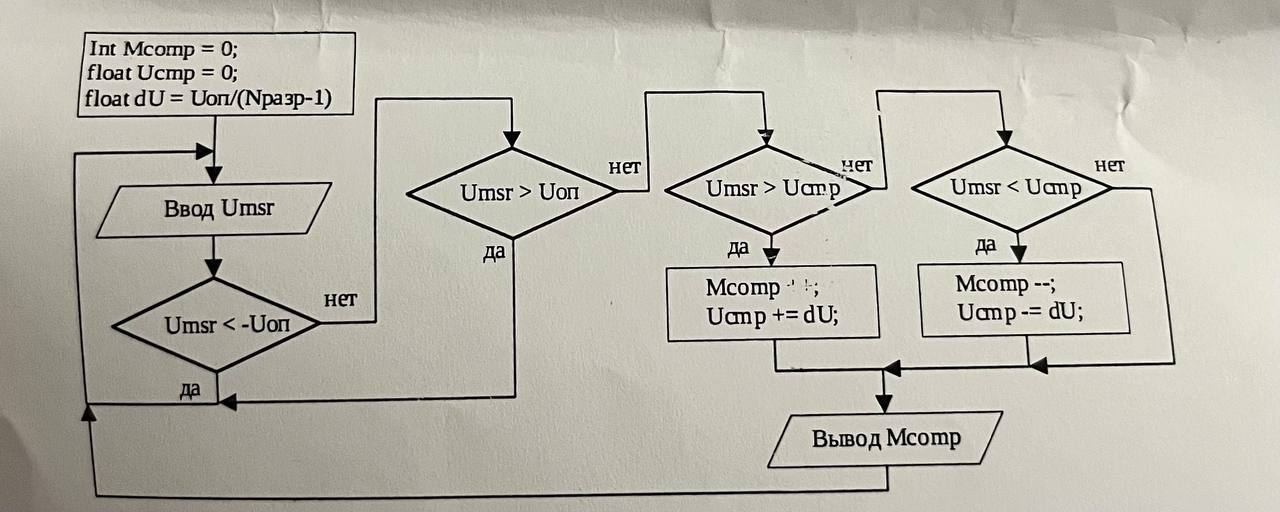
\includegraphics[width=0.8\textwidth]{../alg.jpg}
  \caption{Алгоритм АЦП последовательного изображения}
\end{figure}
\par Где:
\begin{enumerate}
  \item $U_{msr}$ -- входное значение амплитуды
  \item $M_{comp}$ -- выходное значение амплитуды в относительных единицах
  \item $N_{\text{разр}}$ -- количество двоичных разрядов выходного параметра АЦП
  (которое, кстати на практике может быть кринжовым, недвочиным)
  \item $U_{cmp}$ -- текущее(внутреннее) значение напряжения за предыдущий цикл
  \item \item $U_{\text{ОП}}$ -- опорное напряжение
\end{enumerate}

В телеметрии присутствуют еще понятия "татировка" и "калибровка". 
Они описывают ступени процесса обратного преобразования двоичного сигнала в физ. значение,
Но нам необходимо обратное преобразование двоичного сигнала до величины напряжений, 
поступающих с усилительных трактов на вход АЦП, поэтому говорим только о "калибровке".

\newpage
\par Таким образом, подходим к тому, что калибровочный коэффициент,
определяющий уровень амплитуды в вольтах на входе АЦП, имеет формулу:

$$
K_{\text{калибр}} = \frac{U_{\text{ОП}}}{2^{N-1}}
$$
где $U_{\text{ОП}}$ -- опорное напряжение, $\mathit{N}$ -- разрядность 

\par Фазированная антенная решетка(ФАР) представляет собой 
совокупность антенных элементов, размещенных вместе таким образом,
 что диаграмма направленности каждого отдельного элемента
сочетается с диаграммами соседних антенн для формирования 
эффективной диаграммы направленности, называемой \textit{главный лепесток}.
\par\textit{Диаграмма направленности} -- графическое представление
 направленности антенны в трехмерном пространстве. 
\par Сканирующий луч в ФАР формируется алгоритмически 
путем сложения фаз сигнала со всех элементов,
что позволяет выполнять перемещение луча в пространстве 
без задействования поворотных механизмов полотна антенны.

\begin{figure}[h]
  \centering
  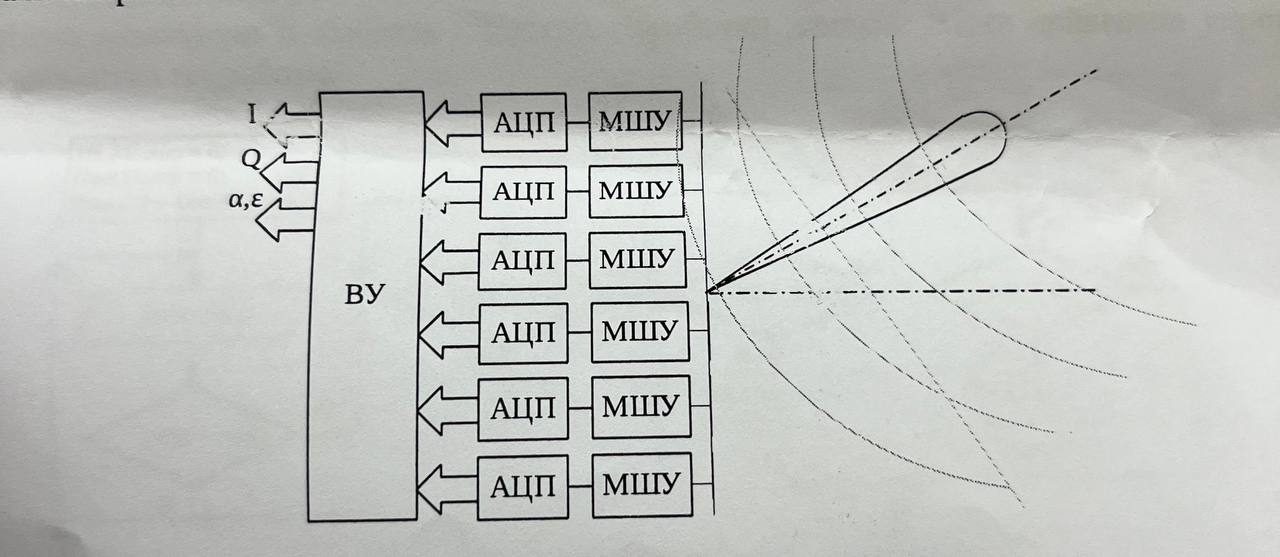
\includegraphics[width=0.8\textwidth]{../phased_array_antenna.jpg}
  \caption{Устройство ФАР}
\end{figure}

\textbf{В качестве заключения:} 

\par\textit{Калибровочный коэффициент} -- постоянная велиична, 
зависимая от разрядности АЦП и уровня опорного напряжения.
\par\textit{Тарировочный коэффициент} может быть отдельным вектором, 
может быть приведенным вместе с коэффициентом усиления антенны

\newpage
\section{Основы ЦОС из книги}
\subsection{In-phase and Quadrature components(Синфаза и квадратура)}

\par Обычно сигнал представляется в виде двух математических схем:
синфазная(I) и квадратурная(Q). Если наш входное сигнал $r(t)$, то 
\[
r(t) = I(t)\cos(w_c t) - Q(t)\sin(w_c t)
\]

\par В приемнике мы преобразуем или уменьшим микширование r(t) 
обратно в наши синфазные и квадратурные сигналы основной 
полосы частот с помощью аналогичного процесса, но в обратном порядке.
Применяя тот же LO со вторым компонентом со сдвигом по фазе к r(t)
с фильтром нижних частот, мы получаем:

\[
I_r(t) = \frac{I(t)}{2}
\]

\[
Q_r(t) = \frac{Q(t)}{2}
\]

\par Сигнал удобно представлять в виде синфазного и квадратурного сигналов,
где синфазный от квадратурного отличается смещение фазы на 90*. 
Часто говорят, что I -- реальный сигнал, Q -- воображаемый

Тогда сам сигнал представляется по формуле:
\[
r(t) = I(t) + jQ(t)  
\]

где
\[
I(t) = A\cos(t)(\omega t+ \phi)  
\]

\[
Q(t) = A\sin(t)(\omega t+ \phi)  
\]

\begin{figure}[h]
  \centering
  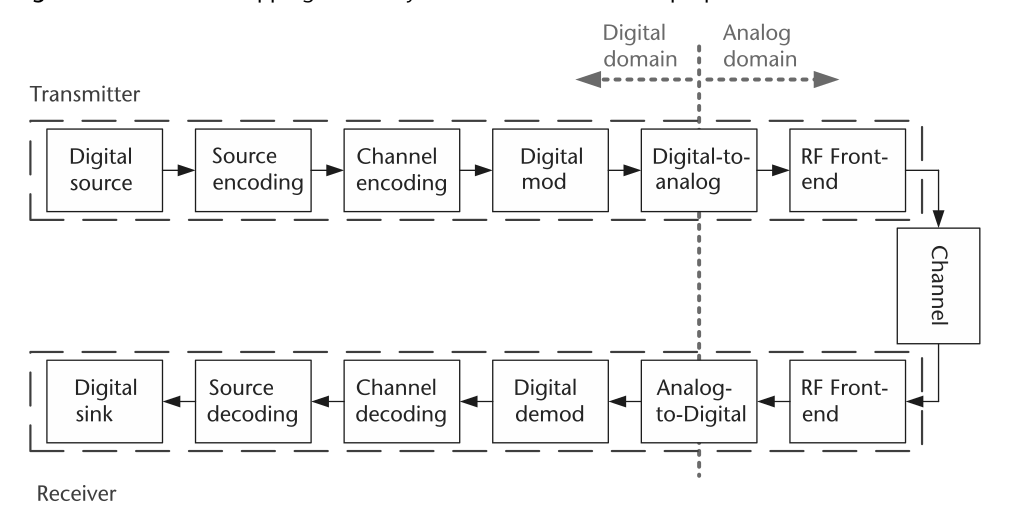
\includegraphics[width=0.8\textwidth]{../transmitter.png}
  \caption{Общее устройство цифрового приемопередатчика}
\end{figure}

\par Все данные предоставляются блоками

\par Базу базовую про модуляцию и тд записывать не буду пока что

\par Есть канальная кодировка и source кодировка данных.
Первая используется для защиты содержания информации. 
Второе же нужно для сжатия данных
(в моем проекте как я понял на сжатие данных пох)
\newpage

\subsection{Энергоэффективность и скорость модуляции}
Чтобы оценить эффективность преобразования бита в символ 
с точки зрения мощности передачи, затрачиваемой на каждый символ,
мы можем использовать показатель энергоэффективности. 
Предположим, мы определили энергию символа s(t) как
$$
E_s = \int_{0}^{T} s^2(t) \partial t,
$$
где T -- период символа

Также можно добавить нудятины и определить затраченную энергию в среднем
$$
\overline{E_s} = \mathit{P(s_1(t))} \cdot \int_{0}^{T} s_1^2(t) + \dots + P(S_M(t))\partial t \cdot \int_{0}^{T} s_M^(t) \partial t,
$$
где $P(s_i(t))$ -- вероятность появления символа $s_i(t)$.

Можно также посчитать энергию на бит:
$$
\overline{E_b} = \frac{\overline{E_s}}{\log_2(M)}
$$

Зачем-то еще в книге дана формула Евклидового расстояния:
\[
d_{\min}^2 = \min_{i \not = j} \int_0^T(s_i(t) - s_j(t))^2 dt
\]

Затем идет вкуснятина -- модуляции:
\begin{enumerate}
  \item PAM
  \item QAM
  \item PSK
\end{enumerate}

На PSK можно остановиться.
\subsection{Phase Shift Keying}

\par На самом деле даже тут не стоит останаливаться надолго, 
потому что я уже выше сам описывал BPSK, а это частный случай PSK

\par Единственное, что энергоэффективность BPSK
\[
\epsilon_{p, BPSK} = \frac{d_{\min}^2 }{\overline{E_b}} = 4 dt
\]


\par Таким образом, формулы для BPSK будут такие:
\[ I_m(t) = A \cos(2 \pi \omega_c t + \pi b(t)) \]
\[ Q_m(t) = A \sin(2 \pi \omega_c t + \pi b(t)) \]

Где \( b(t) \) -- битовая последовательность (0 или 1),
\( A \) -- амплитуда сигнала, \( \omega_c \) -- частота несущей волны.

\par Также еще стоит сказать про BPE(probability bir error) у BPSK:
\par Лень стало, все равно теория

\subsection{ADC (Analog-to-Digital Conversion) and DAC (Digital-to-Digital Conversion)}

\begin{figure}[h]
  \centering
  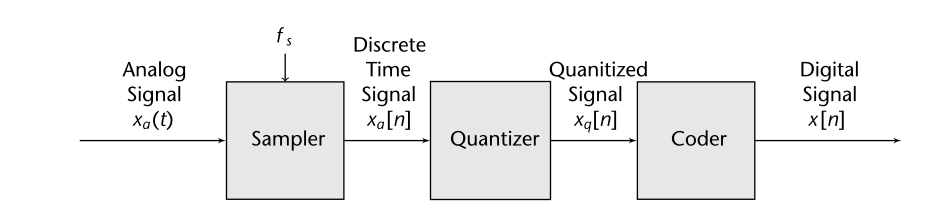
\includegraphics[width=0.8\textwidth]{../adc.png}
  \caption{Основные этапы ADC}
\end{figure}


\end{document}